\documentclass[a4paper,12pt]{article} % добавить leqno в [] для нумерации слева
\usepackage[a4paper,top=1.3cm,bottom=2cm,left=1.5cm,right=1.5cm,marginparwidth=0.75cm]{geometry}
%%% Работа с русским языком
\usepackage{cmap}					% поиск в PDF
\usepackage[warn]{mathtext} 		% русские буквы в фомулах
\usepackage[T2A]{fontenc}			% кодировка
\usepackage[utf8]{inputenc}			% кодировка исходного текста
\usepackage[english,russian]{babel}	% локализация и переносы
\usepackage{multirow}
\usepackage{float}
\restylefloat{table}


%\graphicspath{ {images/}}
\usepackage{graphicx}

\usepackage{wrapfig}
\usepackage{tabularx}

\usepackage{hyperref}
\usepackage[rgb]{xcolor}
\hypersetup{
	colorlinks=true,urlcolor=blue
}

%%% Дополнительная работа с математикой
\usepackage{amsmath,amsfonts,amssymb,amsthm,mathtools} % AMS
\usepackage{icomma} % "Умная" запятая: $0,2$ --- число, $0, 2$ --- перечисление

%% Номера формул
\mathtoolsset{showonlyrefs=true} % Показывать номера только у тех формул, на которые есть \eqref{} в тексте.

%% Шрифты
\usepackage{euscript}	 % Шрифт Евклид
\usepackage{mathrsfs} % Красивый матшрифт

%% Свои команды
\DeclareMathOperator{\sgn}{\mathop{sgn}}

%% Перенос знаков в формулах (по Львовскому)
\newcommand*{\hm}[1]{#1\nobreak\discretionary{}
	{\hbox{$\mathsurround=0pt #1$}}{}}

\date{\today}

\title{Лабораторная работа 1.2.2 Экспериментальная проверка закона вращательного движения на крестообразном маятнике}
\date{}
\begin{document}
\maketitle

\section{Аннотация}
\subsection{Цель работы}
Экспериментально проверить уравнение \eqref{1}, получив зависимость углового ускорения от момента инерции и момента
прикладываемых к системе сил, а также проанализировать влияние
сил трения, действующих в оси вращения.

\subsection{Используемые приборы}
В работе используется крестообразный «маятник» (рис. \ref{pic}), перегрузки разной массы, установка с датчикам и компьютер, с помощью которого происходит управление.

\subsection{Ожидаемые результаты}
Убедимся в справедливости соотношения \eqref{1}, на основе экспериментальных данных получим зависимость углового ускорения от момента инерции и момента прикладываемых к системе сил. Проанализируем влияние на результаты сил трения в оси.

\section{Теоретические сведения}
Закон вращательного движения:
\begin{gather}
	\hat{I}\ddot{\varphi} =\overset{\to}{ M} \label{1},\text{ где } \ddot{\varphi} \equiv \dot{\omega} \equiv \vec\beta, \ \overset{\to}{ M} = \sum_i \overset{ \to}{ M_i}
\end{gather}
\begin{figure}[h!]
\begin{center}
    \label{pic}
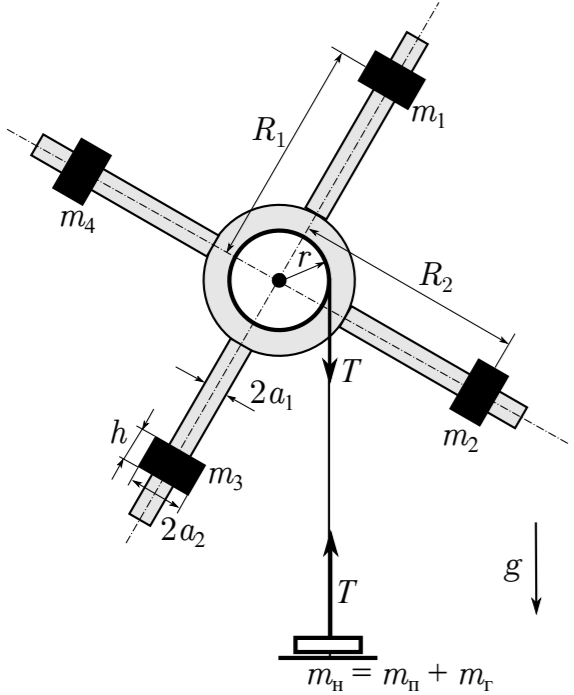
\includegraphics[width=0.5\textwidth]{images/Маятник.png}
\end{center}
\caption{Крестообразный маятник Обербека} \label{маятник}
\end{figure}
На маятник действуют два момента сил: силы натяжения нити $M_T: M_T = rT$, где $r$ - радиус шкива и момент силы трения $ M_\text{тр} $ 
Силу$ T $ выразим из уравнения движения платформы:\begin{gather}
	(m_\text{п} + m_\text{г})\beta r = (m_\text{п} + m_\text{г})g - T \implies M_T =(m_\text{п} + m_\text{г})r(g - \beta r),
\end{gather} где $ m_\text{п} $ -- масса платформы,$ m_\text{г} $ -- масса грузика. 
Пусть $ m_H = (m_\text{п} + m_\text{г}) $ 
Откуда согласно основному уравнению вращательного движения :
\begin{equation}
(I+m_Hr^2)\beta = m_Hgr-M_\text{тр}
\label{M_T}
\end{equation}

Рассмотрим момент силы трения. Его зависимость от скорости не ясна, однако может иметь как составляющую, пропорциональную силе реакции в оси $N$ (сухое трение), так и составляющую, пропорциональную угловой скорости вращения (вязкое трение). Учитывая, что сила реакции уравновешенного маятника равна $ N = m_\text{м}g + T \approx (m_\text{м} + m_\text{н})g \approx m_\text{м}g $,  где$ m_\text{м} $ -- масса маятника. Тогда:
\begin{equation}
M_\text{тр} \simeq \left(1 + \frac{m_H}{m_M}\right) M_0 + \eta \omega \approx M_0 +\eta \omega
\label{трение}
\end{equation} 
где $M_0$ - момент сил трения для покоящегося маятника при нулевой массе подвеса, $m_M$ - масса маятника 

Для расчета момента инерции системы, предположим, что грузы $m_i$ имеют форму полых цилиндров, внутренний и внешний радиус которых известен, образующая h
\begin{equation}
I = I_0 + \sum_{i=1}^4(I_i+m_iR_i^2)
\label{I}
\end{equation}
где $I_0$ - момент инерции системы без грузов, $R_i$ -  расстояние от центров масс грузов до оси вращения
\begin{equation}
I_i = \frac{1}{12}m_ih^2+\frac{1}{4}m_i(a_1^2+a_2^2)
\label{Ii}
\end{equation} -- момент инерции груза относительно оси, проходящей через его центр масс.

\textbf{Используемые приближения:} 
\begin{gather}
	m_\text{м} \gg m_\text{н} \\ 
	m_\text{н} r^2 \ll I \implies M_\text{н} \approx m_\text{н}gr \implies T \approx m_\text{н}g
\end{gather} 

\end{document}